\documentclass[sn-mathphys,Numbered]{sn-jnl}

\usepackage{graphicx}
\usepackage{multirow}
\usepackage{amsmath,amssymb,amsfonts}
\usepackage{booktabs}
\usepackage{url}

\begin{document}

\title[Cold-Start and Steady-State Inference on Heterogeneous Hardware]{Where Does the Time Go? An Empirical Study of Cold-Start and Steady-State Inference Latency Across CPU, Integrated GPU, and Discrete GPU Execution Providers}

\author*[1]{\fnm{Ragul} \sur{K}}
\email{278081@saranathan.ac.in}

\affil*[1]{\orgdiv{Department of Artificial Intelligence and Data Science}, \orgname{Saranathan College of Engineering}, \orgaddress{\city{Tiruchirappalli}, \state{Tamil Nadu}, \country{India}}}

\abstract{
Inference benchmarks commonly emphasize steady-state latency while giving less attention to the time required to initialize an inference session and complete its first execution. This distinction is important for short-lived and interactive edge workloads, where initialization overhead can dominate total execution time. We present an empirical characterization of cold-start and steady-state inference latency across CPU, integrated GPU, and discrete GPU execution providers on a consumer laptop using native C++17, ONNX Runtime 1.20.1, and DirectML. We evaluate SqueezeNet 1.1 and MobileNetV2 using 160 isolated benchmark trials. The results show substantial backend-dependent cold-start costs. For example, the measured cold-start total for SqueezeNet is 28.78 ms on a four-thread CPU and 288.49 ms on the NVIDIA RTX 3050, whereas the corresponding steady-state medians are 2.372 ms and 1.035 ms. We derive a workload-length break-even model and estimate that the RTX 3050 requires 196 completed SqueezeNet frames to compensate for its higher cold-start cost under the measured median-latency model. No GPU configuration crosses over against the four-thread CPU for MobileNetV2. We also examine an asynchronous CPU--GPU dispatcher through two separate 40-trial datasets. The dispatcher results expose the importance of correct backend-specific performance calibration and are reported as diagnostic evidence rather than as a demonstrated speedup. These findings show why cold-start and steady-state measurements should be considered together when selecting execution providers for edge inference.
}

\keywords{Edge Inference \and Cold-Start Latency \and DirectML \and Heterogeneous Computing \and ONNX Runtime \and GPU Scheduling}

\maketitle

\section{Introduction}

Deep neural network inference increasingly runs directly on client devices and edge systems. Such environments include laptops and compact workstations that combine multi-core CPUs, integrated GPUs, and discrete GPUs. Applications using these devices include interactive vision, local analytics, and privacy-preserving inference \cite{wu2019machine}. Frameworks such as ONNX Runtime provide a common interface for executing models across different hardware backends \cite{onnxruntime2024}.

Many inference benchmarks emphasize steady-state execution by measuring repeated model runs after initialization and warm-up. However, a newly launched application must first load and initialize its inference session and complete its first inference. Depending on the execution provider, these operations may involve graph optimization, device initialization, resource allocation, and backend-specific preparation. Consequently, a backend with lower steady-state latency does not necessarily provide the lowest completion time for a short workload.

This distinction is particularly relevant to edge applications that process a finite number of frames before terminating or becoming idle. A discrete GPU may provide faster repeated inference but incur a substantial initial cost. A CPU may therefore remain preferable for short workloads even when its steady-state latency is higher.

This paper investigates the relationship between cold-start and steady-state inference latency across CPU, integrated GPU (iGPU), and discrete GPU (dGPU) execution providers on a consumer laptop. We use SqueezeNet 1.1 \cite{iandola2016squeezenet} and MobileNetV2 \cite{sandler2018mobilenetv2} as representative lightweight vision workloads.

The contributions are as follows:

\begin{enumerate}
    \item \textbf{Cold-start characterization:} We measure session creation, first-inference latency, and steady-state latency across four execution configurations: one-thread CPU, four-thread CPU, Intel UHD integrated GPU, and NVIDIA RTX 3050 discrete GPU. The evaluation comprises 160 isolated trials.

    \item \textbf{Workload-length break-even model:} We formulate a closed-form model that estimates the minimum number of inference frames required for a GPU backend to compensate for its additional cold-start cost relative to CPU execution.

    \item \textbf{Dispatcher implementation and diagnostic evaluation:} We implement an asynchronous CPU--GPU execution dispatcher in C++17 and evaluate its behavior using two separate 40-trial datasets. The results demonstrate the practical importance of correct backend-specific latency estimates and identify limitations that must be addressed before claiming a scheduling benefit.
\end{enumerate}

\section{Methodology and Experimental Setup}

\subsection{Hardware and Software Environment}

All experiments were conducted on an Infinix GT Book laptop running Windows 11. The system configuration was:

\begin{itemize}
    \item \textbf{CPU:} Intel Core i5-12450H, with four Performance-cores, four Efficiency-cores, and twelve logical threads.
    \item \textbf{Integrated GPU:} Intel UHD Graphics, enumerated as DirectML device 0.
    \item \textbf{Discrete GPU:} NVIDIA GeForce RTX 3050 6GB Laptop GPU, enumerated as DirectML device 1.
    \item \textbf{Runtime:} ONNX Runtime 1.20.1 with the DirectML execution provider.
    \item \textbf{Implementation:} Native C++17 benchmark programs compiled using MinGW-w64 GCC 16.2.0 with optimization enabled.
\end{itemize}

The DirectML device mapping was established using adapter enumeration. Device identifiers are provider-specific identifiers and should not be interpreted as universal GPU identifiers.

\subsection{Workload Selection}

We evaluate two image-classification models with different computational structures:

\begin{itemize}
    \item \textbf{SqueezeNet 1.1:} A compact convolutional architecture using Fire modules and a combination of $1 \times 1$ and $3 \times 3$ convolutions \cite{iandola2016squeezenet}.
    \item \textbf{MobileNetV2:} An architecture using inverted residual blocks and depthwise-separable convolutions \cite{sandler2018mobilenetv2}.
\end{itemize}

Both models are evaluated using a fixed input shape of $1 \times 3 \times 224 \times 224$ with FP32 input tensors. The same deterministic input-generation procedure is used across the benchmark configurations.

\subsection{Cold-Start Measurement Protocol}

Each baseline trial runs in an independent operating-system process. The benchmark creates an ONNX Runtime session, executes one first inference, and then performs 100 warm inference iterations.

We record:

\begin{itemize}
    \item $T_{\mathrm{create}}$: time required to create the inference session.
    \item $T_{\mathrm{first}}$: execution time of the first inference after session creation.
    \item $t_{\mathrm{steady}}$: median latency of the warm inference iterations.
    \item $t_{p95}$: 95th-percentile latency of the warm inference iterations.
\end{itemize}

For each of the two models, we execute 20 trials on each of four configurations, resulting in 160 baseline trials. The configurations are CPU with one thread, CPU with four threads, Intel UHD integrated GPU, and NVIDIA RTX 3050 discrete GPU.

We report medians and interquartile ranges (IQR) for repeated measurements. The reported cold-start total is calculated as the sum of the median session-creation time and the median first-inference time:

\begin{equation}
T_{\mathrm{cold}} =
\operatorname{median}(T_{\mathrm{create}})
+
\operatorname{median}(T_{\mathrm{first}}).
\end{equation}

This quantity is a sum of component medians and is not the median of per-trial total latency.

The benchmark records an output tensor checksum as a numerical diagnostic. The checksum is not treated as a formal cross-backend numerical-equivalence test.

\subsection{Dispatcher Experiment Protocol}

In addition to the baseline benchmark, we evaluate an asynchronous C++ dispatcher that creates a CPU session on the main thread while a background worker initializes a DirectML session and performs a warm-up inference.

The dispatcher records time-to-first-inference (TTFI), GPU initialization duration, CPU and GPU phase latencies, switch frame, workload wall time, and process wall time.

Two separate dispatcher datasets are retained: an earlier implementation with 40 trials and a subsequent dispatcher implementation with 40 trials. They are not combined with the 160 baseline trials or with each other. The subsequent experiment uses 10 trials for each of four model--device configurations and an 800-frame workload.

\section{Analytical Crossover Model}

\subsection{Break-Even Formulation}

Let $T_{\mathrm{cold}}^{(b)}$ denote the time to complete the first inference on backend $b$, and let $t_{\mathrm{steady}}^{(b)}$ denote its median steady-state per-frame latency.

For a workload of $N$ frames, the modeled cumulative execution time is:

\begin{equation}
C^{(b)}(N) =
T_{\mathrm{cold}}^{(b)}
+
(N-1)t_{\mathrm{steady}}^{(b)}.
\end{equation}

We compare a GPU backend against the four-thread CPU configuration. The GPU is faster over the complete workload when:

\begin{equation}
T_{\mathrm{cold}}^{(G)}
+
(N-1)t_{\mathrm{steady}}^{(G)}
<
T_{\mathrm{cold}}^{(C)}
+
(N-1)t_{\mathrm{steady}}^{(C)}.
\end{equation}

A finite crossover is possible only if:

\begin{equation}
t_{\mathrm{steady}}^{(G)}
<
t_{\mathrm{steady}}^{(C)}.
\end{equation}

For this case, define:

\begin{equation}
r =
\frac{
T_{\mathrm{cold}}^{(G)}-T_{\mathrm{cold}}^{(C)}
}{
t_{\mathrm{steady}}^{(C)}-t_{\mathrm{steady}}^{(G)}
}.
\end{equation}

The smallest integer workload size satisfying the strict inequality is:

\begin{equation}
N^* =
\begin{cases}
\max(1,\lfloor r \rfloor+2),
&
t_{\mathrm{steady}}^{(G)}
<
t_{\mathrm{steady}}^{(C)},\\[6pt]
\text{No crossover},
&
\text{otherwise}.
\end{cases}
\end{equation}

This threshold is an analytical estimate derived from measured medians. It does not account for changing thermal conditions, runtime contention, or variation in individual inference latency.

\section{Experimental Results}

\subsection{Cold-Start and Steady-State Latency}

Table~\ref{tab:coldstart} presents the baseline measurements across 160 trials. All latency values are in milliseconds.

\begin{table}[ht]
\caption{Baseline cold-start and steady-state measurements. Session creation is reported as median (IQR). Other columns report medians.}
\label{tab:coldstart}
\centering
\small
\begin{tabular}{@{}llrrrrrr@{}}
\toprule
Model & Backend & Create (IQR) & First & Cold & Steady & $p_{95}$ & Gap \\
\midrule
\multirow{4}{*}{SqueezeNet 1.1}
& CPU (1T) & 23.75 (1.53) & 9.16 & 32.91 & 7.95 & 9.71 & 24.77 \\
& CPU (4T) & 24.79 (1.66) & 3.98 & 28.78 & 2.37 & 2.51 & 26.50 \\
& Intel UHD & 62.96 (10.84) & 5.19 & 68.15 & 3.89 & 4.16 & 64.32 \\
& RTX 3050 & 285.83 (12.17) & 2.66 & 288.49 & 1.03 & 1.16 & 287.55 \\
\midrule
\multirow{4}{*}{MobileNetV2}
& CPU (1T) & 41.07 (4.13) & 9.32 & 50.39 & 8.66 & 10.74 & 41.47 \\
& CPU (4T) & 42.66 (2.84) & 3.82 & 46.48 & 2.72 & 2.90 & 43.73 \\
& Intel UHD & 85.72 (10.21) & 44.71 & 130.43 & 12.47 & 13.35 & 118.75 \\
& RTX 3050 & 96.42 (7.24) & 237.83 & 334.25 & 4.07 & 4.72 & 331.61 \\
\bottomrule
\end{tabular}
\end{table}

Figure~\ref{fig:breakdown} compares cold-start totals with steady-state median latency.

\begin{figure}[ht]
\centering
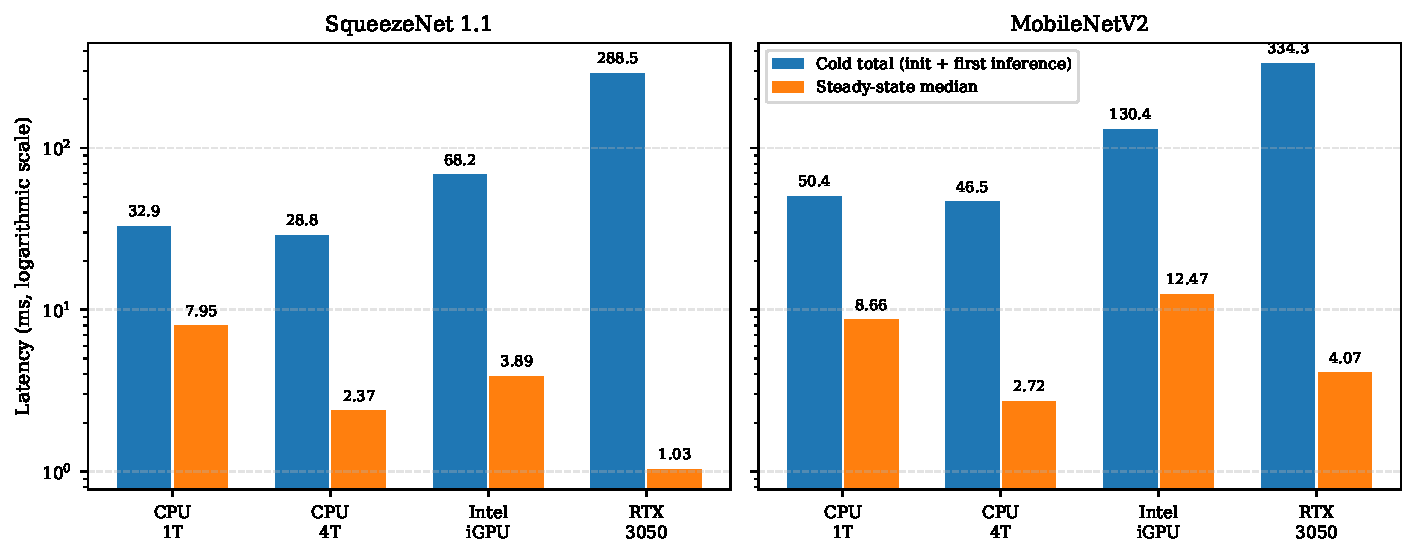
\includegraphics[width=0.98\textwidth]{figures/fig1_coldstart_breakdown.pdf}
\caption{Cold-start total and steady-state median latency across CPU, Intel UHD integrated GPU, and NVIDIA RTX 3050 discrete GPU configurations. The vertical axis uses a logarithmic scale.}
\label{fig:breakdown}
\end{figure}

Three observations emerge from the baseline measurements.

\begin{enumerate}
    \item \textbf{Backend-dependent initialization cost:} SqueezeNet on the RTX 3050 has a cold-start total of 288.49 ms, despite a steady-state median of only 1.035 ms. For MobileNetV2 on the RTX 3050, the cold-start total is 334.25 ms, with 237.83 ms spent in the first inference. The measurements show that initialization and first-execution costs are distinct and model-dependent.

    \item \textbf{Steady-state backend differences:} For SqueezeNet, the RTX 3050 achieves a steady-state median of 1.035 ms, compared with 2.372 ms on the four-thread CPU. Intel UHD achieves 3.889 ms. For MobileNetV2, the four-thread CPU is faster than both GPU configurations: 2.724 ms compared with 4.074 ms on the RTX 3050 and 12.471 ms on Intel UHD.

    \item \textbf{Model-dependent first-inference behavior:} The first-inference median for MobileNetV2 on the RTX 3050 is 237.83 ms, considerably higher than its session-creation median of 96.42 ms. In contrast, SqueezeNet on the RTX 3050 has a first-inference median of 2.66 ms. Thus, session creation alone is insufficient to characterize the complete cold-start cost.
\end{enumerate}

\subsection{Crossover Analysis}

Table~\ref{tab:crossover} reports the break-even results calculated against CPU execution with four threads.

\begin{table}[ht]
\caption{Modeled GPU break-even workload sizes relative to CPU (4T). A finite value denotes the smallest integer frame count at which modeled GPU completion time is strictly lower.}
\label{tab:crossover}
\centering
\small
\begin{tabular}{@{}llrrrr@{}}
\toprule
Model & GPU & CPU Cold & GPU Cold & CPU Steady & GPU Steady \\
\midrule
SqueezeNet 1.1 & Intel UHD & 28.78 & 68.15 & 2.372 & 3.889 \\
SqueezeNet 1.1 & RTX 3050 & 28.78 & 288.49 & 2.372 & 1.035 \\
MobileNetV2 & Intel UHD & 46.48 & 130.43 & 2.724 & 12.471 \\
MobileNetV2 & RTX 3050 & 46.48 & 334.25 & 2.724 & 4.074 \\
\bottomrule
\end{tabular}
\end{table}

The resulting break-even thresholds are:

\begin{itemize}
    \item \textbf{SqueezeNet on RTX 3050:} The modeled crossover occurs at 196 frames. Its lower steady-state latency eventually compensates for the higher initial cost.
    \item \textbf{SqueezeNet on Intel UHD:} No crossover occurs because its measured steady-state latency is higher than CPU (4T).
    \item \textbf{MobileNetV2 on both GPUs:} No crossover occurs because neither GPU has a lower steady-state median than CPU (4T).
\end{itemize}

Figure~\ref{fig:crossover} visualizes the modeled cumulative latency over 1,000 frames. The curves are calculated from the baseline cold-start and steady-state medians; they are not measurements of a continuously running dispatcher.

\begin{figure}[ht]
\centering
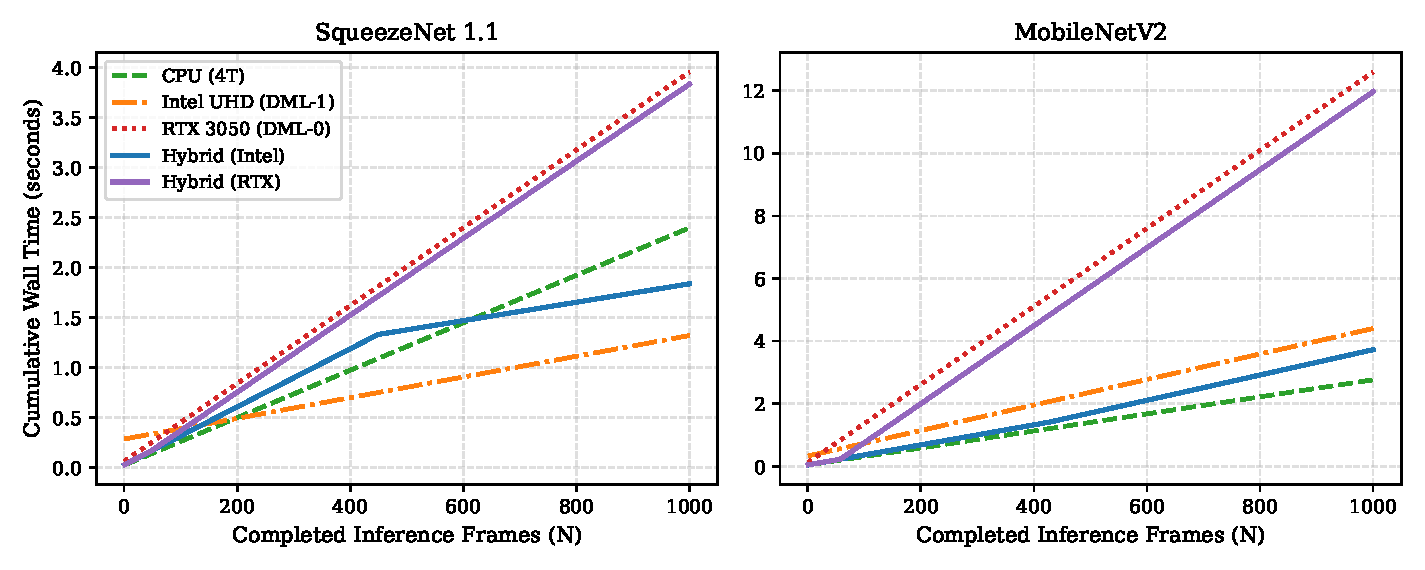
\includegraphics[width=0.98\textwidth]{figures/fig2_cumulative_crossover.pdf}
\caption{Modeled cumulative execution time over 1,000 inference frames using measured cold-start and steady-state medians. The SqueezeNet RTX 3050 curve crosses below CPU (4T) at 196 frames. No GPU crossover is observed for MobileNetV2.}
\label{fig:crossover}
\end{figure}

\subsection{Asynchronous Dispatcher Evaluation}

We implemented a dispatcher that initializes the CPU session on the main thread while a background worker initializes and warms a DirectML session. The dispatcher uses backend-specific latency estimates to determine whether GPU execution is considered profitable and when to hand off execution.

The subsequent 40-trial experiment is summarized in Table~\ref{tab:dispatcher}. Each configuration contains 10 trials. A value of ``--'' indicates that no GPU phase was recorded because the dispatcher did not select GPU execution.

\begin{table}[ht]
\caption{Subsequent asynchronous dispatcher experiment: median values across 10 trials per model--device configuration. TTFI is measured from dispatcher application start to first completed inference.}
\label{tab:dispatcher}
\centering
\small
\begin{tabular}{@{}llrrrrl@{}}
\toprule
Model & GPU & TTFI & Switch & GPU Init & CPU Phase & GPU Phase & Decision \\
\midrule
SqueezeNet 1.1 & Intel UHD & 48.87 & 42.5 & 234.11 & 4.09 & 4.63 & Selected \\
SqueezeNet 1.1 & RTX 3050 & 45.58 & -- & -- & 2.92 & -- & Skipped \\
MobileNetV2 & Intel UHD & 75.06 & -- & -- & 3.59 & -- & Skipped \\
MobileNetV2 & RTX 3050 & 73.08 & -- & -- & 3.56 & -- & Skipped \\
\bottomrule
\end{tabular}
\end{table}

The dispatcher selected GPU execution only for SqueezeNet on Intel UHD. In that configuration, the median GPU phase latency was 4.63 ms, compared with 4.09 ms for the CPU phase. Thus, the observed GPU phase was approximately 13.2\% slower than the CPU phase.

This selection is inconsistent with the baseline measurements, which show that Intel UHD has a steady-state median of 3.889 ms for SqueezeNet, compared with 2.372 ms on CPU (4T). Inspection of the dispatcher calibration values identified an inverted device-to-estimate mapping in the tested configuration. The dispatcher assigned the lower SqueezeNet GPU estimate to DirectML device 0, which is Intel UHD, rather than to device 1, which is the RTX 3050.

Consequently, this experiment does not demonstrate a performance improvement from the dispatcher. Instead, it illustrates that an estimate-guided scheduler can make an incorrect offloading decision when its device-specific calibration is inconsistent with the actual hardware mapping.

Figure~\ref{fig:dispatcher} presents the observed TTFI and phase-latency diagnostics for the subsequent dispatcher experiment.

\begin{figure}[ht]
\centering
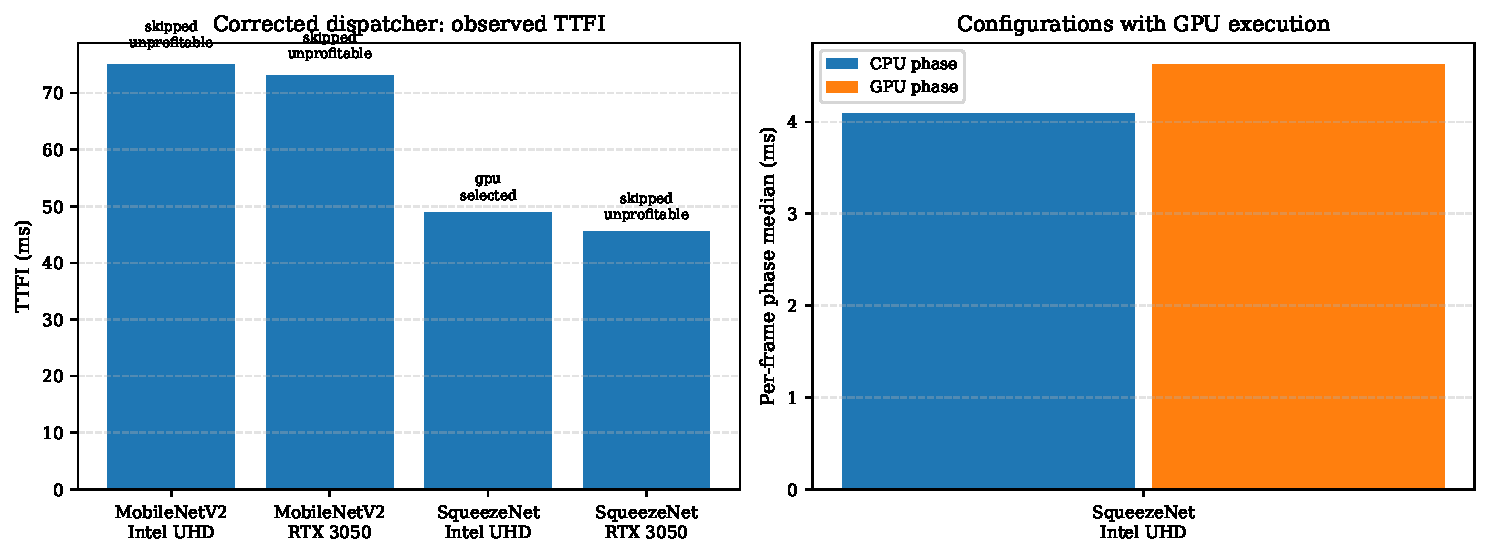
\includegraphics[width=0.98\textwidth]{figures/fig3_hybrid_ttfi_comparison.pdf}
\caption{Diagnostic measurements from the subsequent asynchronous dispatcher experiment. The left panel reports observed TTFI and decisions; the right panel compares CPU and GPU phase medians for the selected configuration. These measurements are not interpreted as a TTFI speedup over the baseline.}
\label{fig:dispatcher}
\end{figure}

An earlier 40-trial dispatcher dataset is also retained in the repository. It belongs to an earlier implementation and is not pooled with the subsequent experiment. Differences in implementation and measurement behavior prevent treating the two datasets as repeated measurements of an identical dispatcher.

\section{Threats to Validity}

The results should be interpreted in light of the following limitations:

\begin{itemize}
    \item \textbf{Single hardware platform:} All experiments were performed on one laptop containing an Intel Core i5-12450H, Intel UHD integrated graphics, and an RTX 3050 6GB Laptop GPU. The numerical results may differ on other processors, GPUs, drivers, and memory configurations.

    \item \textbf{Limited workload coverage:} Only two image-classification models were evaluated, using batch size one and FP32 inputs. Larger batches, transformer models, and compute-intensive workloads may produce different backend rankings.

    \item \textbf{Execution provider scope:} GPU measurements use ONNX Runtime with DirectML. The findings should not be generalized directly to CUDA, TensorRT, or other execution providers.

    \item \textbf{Median-based crossover model:} The break-even equation uses median cold-start and steady-state measurements. It does not model tail-latency constraints, dynamic workload changes, or the distribution of per-frame latency.

    \item \textbf{Dispatcher calibration:} The subsequent dispatcher experiment exposed a device-specific calibration mapping error. Its results therefore serve as diagnostic evidence, not as proof that the implemented scheduler improves inference performance.

    \item \textbf{Concurrent execution effects:} Background GPU initialization and CPU inference may contend for host CPU and memory resources. The dispatcher measurements may therefore differ from isolated baseline measurements.

    \item \textbf{Cold-start interpretation:} Session creation and first-inference measurements capture observable runtime costs. The experiment does not independently profile shader compilation, graph optimization, memory allocation, or individual DirectML internal operations. These activities should not be assigned separate causal durations based solely on the measured timings.
\end{itemize}

\section{Conclusion}

This study characterized cold-start and steady-state inference latency across CPU, integrated GPU, and discrete GPU execution providers on a consumer laptop. Across 160 isolated baseline trials, the measurements showed that session creation and first-inference costs can substantially change the relative performance of execution backends.

For SqueezeNet 1.1, the RTX 3050 achieved a steady-state median of 1.035 ms compared with 2.372 ms on CPU (4T), but its cold-start total was 288.49 ms compared with 28.78 ms on CPU. A median-based analytical model estimated that 196 frames are required for the RTX 3050 to become faster in cumulative completion time. For MobileNetV2, neither GPU configuration achieved a lower steady-state median than CPU (4T), and no crossover was predicted.

The asynchronous dispatcher experiments further highlighted the importance of accurate backend-specific calibration. The subsequent experiment exposed an inverted device-to-estimate mapping that caused an unprofitable GPU selection. We therefore do not claim a dispatcher speedup from these measurements.

Overall, the results demonstrate that reporting steady-state inference latency alone can provide an incomplete picture of edge inference performance. Cold-start costs, workload length, model architecture, and correct hardware identification should all be considered when selecting an execution backend.

\section*{Data and Code Availability}

The C++17 benchmark harness, asynchronous dispatcher implementations, experiment scripts, raw telemetry datasets, analysis script, and figure-generation outputs are available at:

\url{https://github.com/ragulk143/ort-directml-coldstart}

The repository contains 160 baseline trials, 40 trials from the earlier dispatcher implementation, and 40 trials from the subsequent dispatcher experiment. These datasets are retained separately.

\bibliography{refs}

\end{document}
